% Q14 -- Design for Testability (DFT) techniques: tree with three approaches.
% Root DFT -> {Ad hoc testing, Scan-based approaches, Built-In Self-Test (BIST)}.
\documentclass[border=10pt]{standalone}
\usepackage{tikz}
\usetikzlibrary{arrows.meta,positioning}
\begin{document}
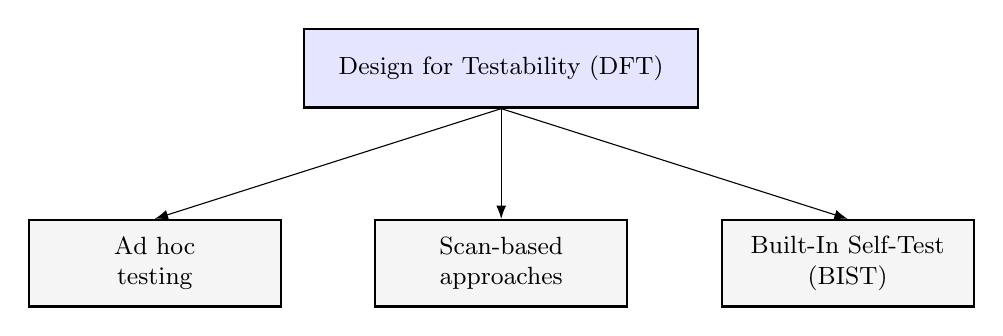
\begin{tikzpicture}[>=Latex, font=\small,
  root/.style={draw, thick, fill=blue!10, minimum width=5cm, minimum height=1cm, align=center},
  child/.style={draw, thick, fill=gray!8, minimum width=3.2cm, minimum height=1.1cm, align=center}]
\node[root] (r) {Design for Testability (DFT)};
\node[child, below=1.4cm of r.south, xshift=-4.4cm] (a) {Ad hoc\\ testing};
\node[child, below=1.4cm of r.south] (b) {Scan-based\\ approaches};
\node[child, below=1.4cm of r.south, xshift=4.4cm] (c) {Built-In Self-Test\\ (BIST)};
\draw[->] (r.south) -- (a.north);
\draw[->] (r.south) -- (b.north);
\draw[->] (r.south) -- (c.north);
\end{tikzpicture}
\end{document}
